\documentclass[handout,t,compress]{beamer}
\usetheme{Singapore}

\sloppy
%\usepackage[scaled]{helvet}
%\usepackage{eulervm}

\usepackage{fp-eval}
\usepackage{hyperref}
\usepackage{fancyvrb}
%\usepackage{pstricks,pst-node,pst-tree,pst-plot,pst-3dplot,multido}
\usepackage{graphicx}
\usepackage{multicol}

\usepackage{alltt}

\newcommand{\bi}{\begin{itemize}}
\newcommand{\li}{\item}
\newcommand{\ei}{\end{itemize}}

\newcommand{\sect}[1]{\begin{frame}[fragile]{#1}}

\definecolor{orange}{rgb}{1,.5,0}
\definecolor{pink}{rgb}{1,.75,.75}
\definecolor{ltblue}{rgb}{.75,.75,1}

\newcommand{\be}{\begin{eqnarray*}}
\newcommand{\ee}{\end{eqnarray*}}

\AtBeginSection[]
{
\bframe{Outline}
\tableofcontents[currentsection]
\end{frame}
}

\title{Intro to Game AI}
\author{CSCI 321}
\institute{WWU}

\begin{document}



\sect{~}
\titlepage
\end{frame}

\sect{Strong AI {\em vs.} Weak AI}
\bi
\li Strong AI: \\ Create programs that think and act intelligently.
\li Weak AI: \\ Create programs that do things intelligent humans do:
\bi
\li play chess
\li drive a car
\li perform surgery
\li predict the weather
\li ...
\ei
It doesn't matter how.
\ei
\end{frame}

\sect{Academic AI {\em vs.} Game AI}
\bi
\li Academic AI 
\bi
\li focuses on optimal performance.
\li usually not real-time.
\ei
\li Game AI
\bi
\li very limited resources (graphics is king)
\li make an engaging opponent
\li can't be too stupid
\li can't be smarter than the player
\li artificial stupidity
\ei 
\ei

\end{frame}

\sect{The Illusion of Intelligence}
\bi
\li Halo playtesting: 

\li When designers gave the NPCs very low hit points:
\begin{tabular}{rl}
AI too easy: & 36\% \\
AI very intelligent: & 8\%
\end{tabular}
\li When designers gave the NPCs very high hit points:
\begin{tabular}{rl}
AI too easy: & 0\% \\
AI very intelligent: & 43\%
\end{tabular}
\ei


\end{frame}

\sect{Acting human gives illusion of higher intelligence}
\bi
\li Act startled when player enters room
\li Look around when there's a noise
\li Track neighboring agents when they move
\ei

\end{frame}

\sect{Acting stupid destroys all faith in AI}
\bi
\li Running into walls
\li Getting stuck in corners
\li Not reacting to ``obvious'' stimuli
\ei

\end{frame}

\sect{Getting caught cheating destroys all faith in AI}
\bi
\li Instant reactions
\li Seeing through walls
\li Perfect aim
\li Hearing everything
\li Getting bigger rewards for less gold
\li Obviously more hit points
\ei
\end{frame}

\sect{The Uncanny Valley}


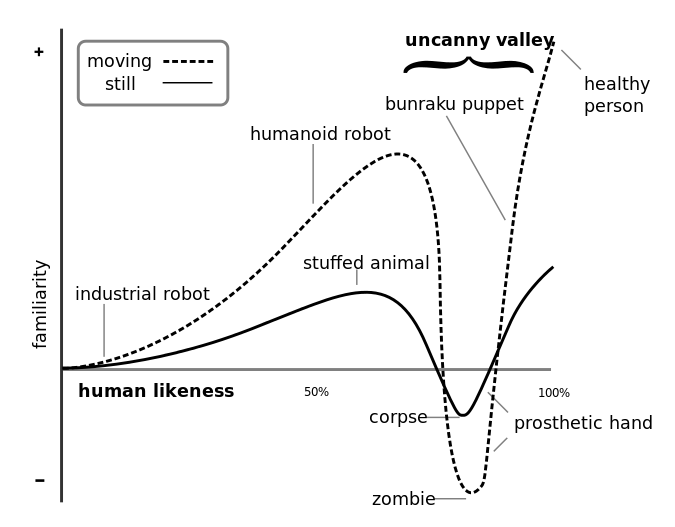
\includegraphics[scale=0.33]{uncannyvalley.png}

\hfill
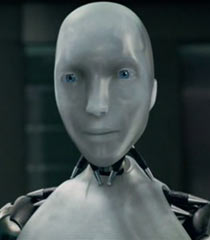
\includegraphics[scale=0.25]{irobot.jpg}
\hfill
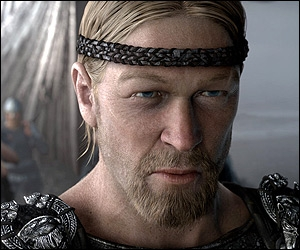
\includegraphics[scale=0.25]{beowulf.jpg}
\hfill
\mbox{}

\end{frame}

\end{document}
